\documentclass[12pt]{article}

%\usepackage{algo}
\usepackage{tikz,fullpage,url,amssymb,amsmath,epsfig,color,xspace,alltt,mathtools}
\usetikzlibrary{shapes,chains,positioning}
\usepackage[pdftitle={CS 240 Assignment 2},%
pdfsubject={University of Waterloo, CS 240, Fall 2021},%
pdfauthor={MP}]{hyperref}
%\RequirePackage{pstricks,pst-node,pst-tree} % draw trees, requires using xetex
\newlength{\nodeLength}
\newcommand{\Node}{A}
\newcommand{\setnode}[1]{
	\settowidth{\nodeLength}{#1}
	\renewcommand{\Node}[1]{
		\Tcircle[name=#1]{\makebox[\nodeLength]{##1}}
	}
}
\setnode{99}

\newcommand{\ceil}[1]{\left\lceil #1 \right\rceil}
\newcommand{\floor}[1]{\left\lfloor #1 \right\rfloor}
\renewcommand{\thesubsection}{Problem \arabic{subsection}}

\begin{document}
	
	a)
	
	\begin{center}
		{\Large\bf Problem 7}\\
		\vspace{3mm}
	\end{center}
	
	\definecolor{care}{rgb}{0,0,0}
	\def\question#1{\item[\bf #1.]}
	\def\part#1{\item[\bf #1)]}
	\newcommand{\pc}[1]{\mbox{\textbf{#1}}} % pseudocode
	
	
	
	%%%%%%%%%%%%%%%%%%%%%%%%%%%%%%%%%%%%%%%%%%%%%%%%%%%%%%%%%%%%%
	
	\begin{tabular}{ | l || c  | c | c | c | c |} \hline
		Key & 7 & 42 & 27 & 31 & 10  \\ \hline
		Height & 0 & 2 & 0  & 3 & 1 \\ \hline
	\end{tabular}
	\begin{figure}[tbhp]
		\begin{center}
			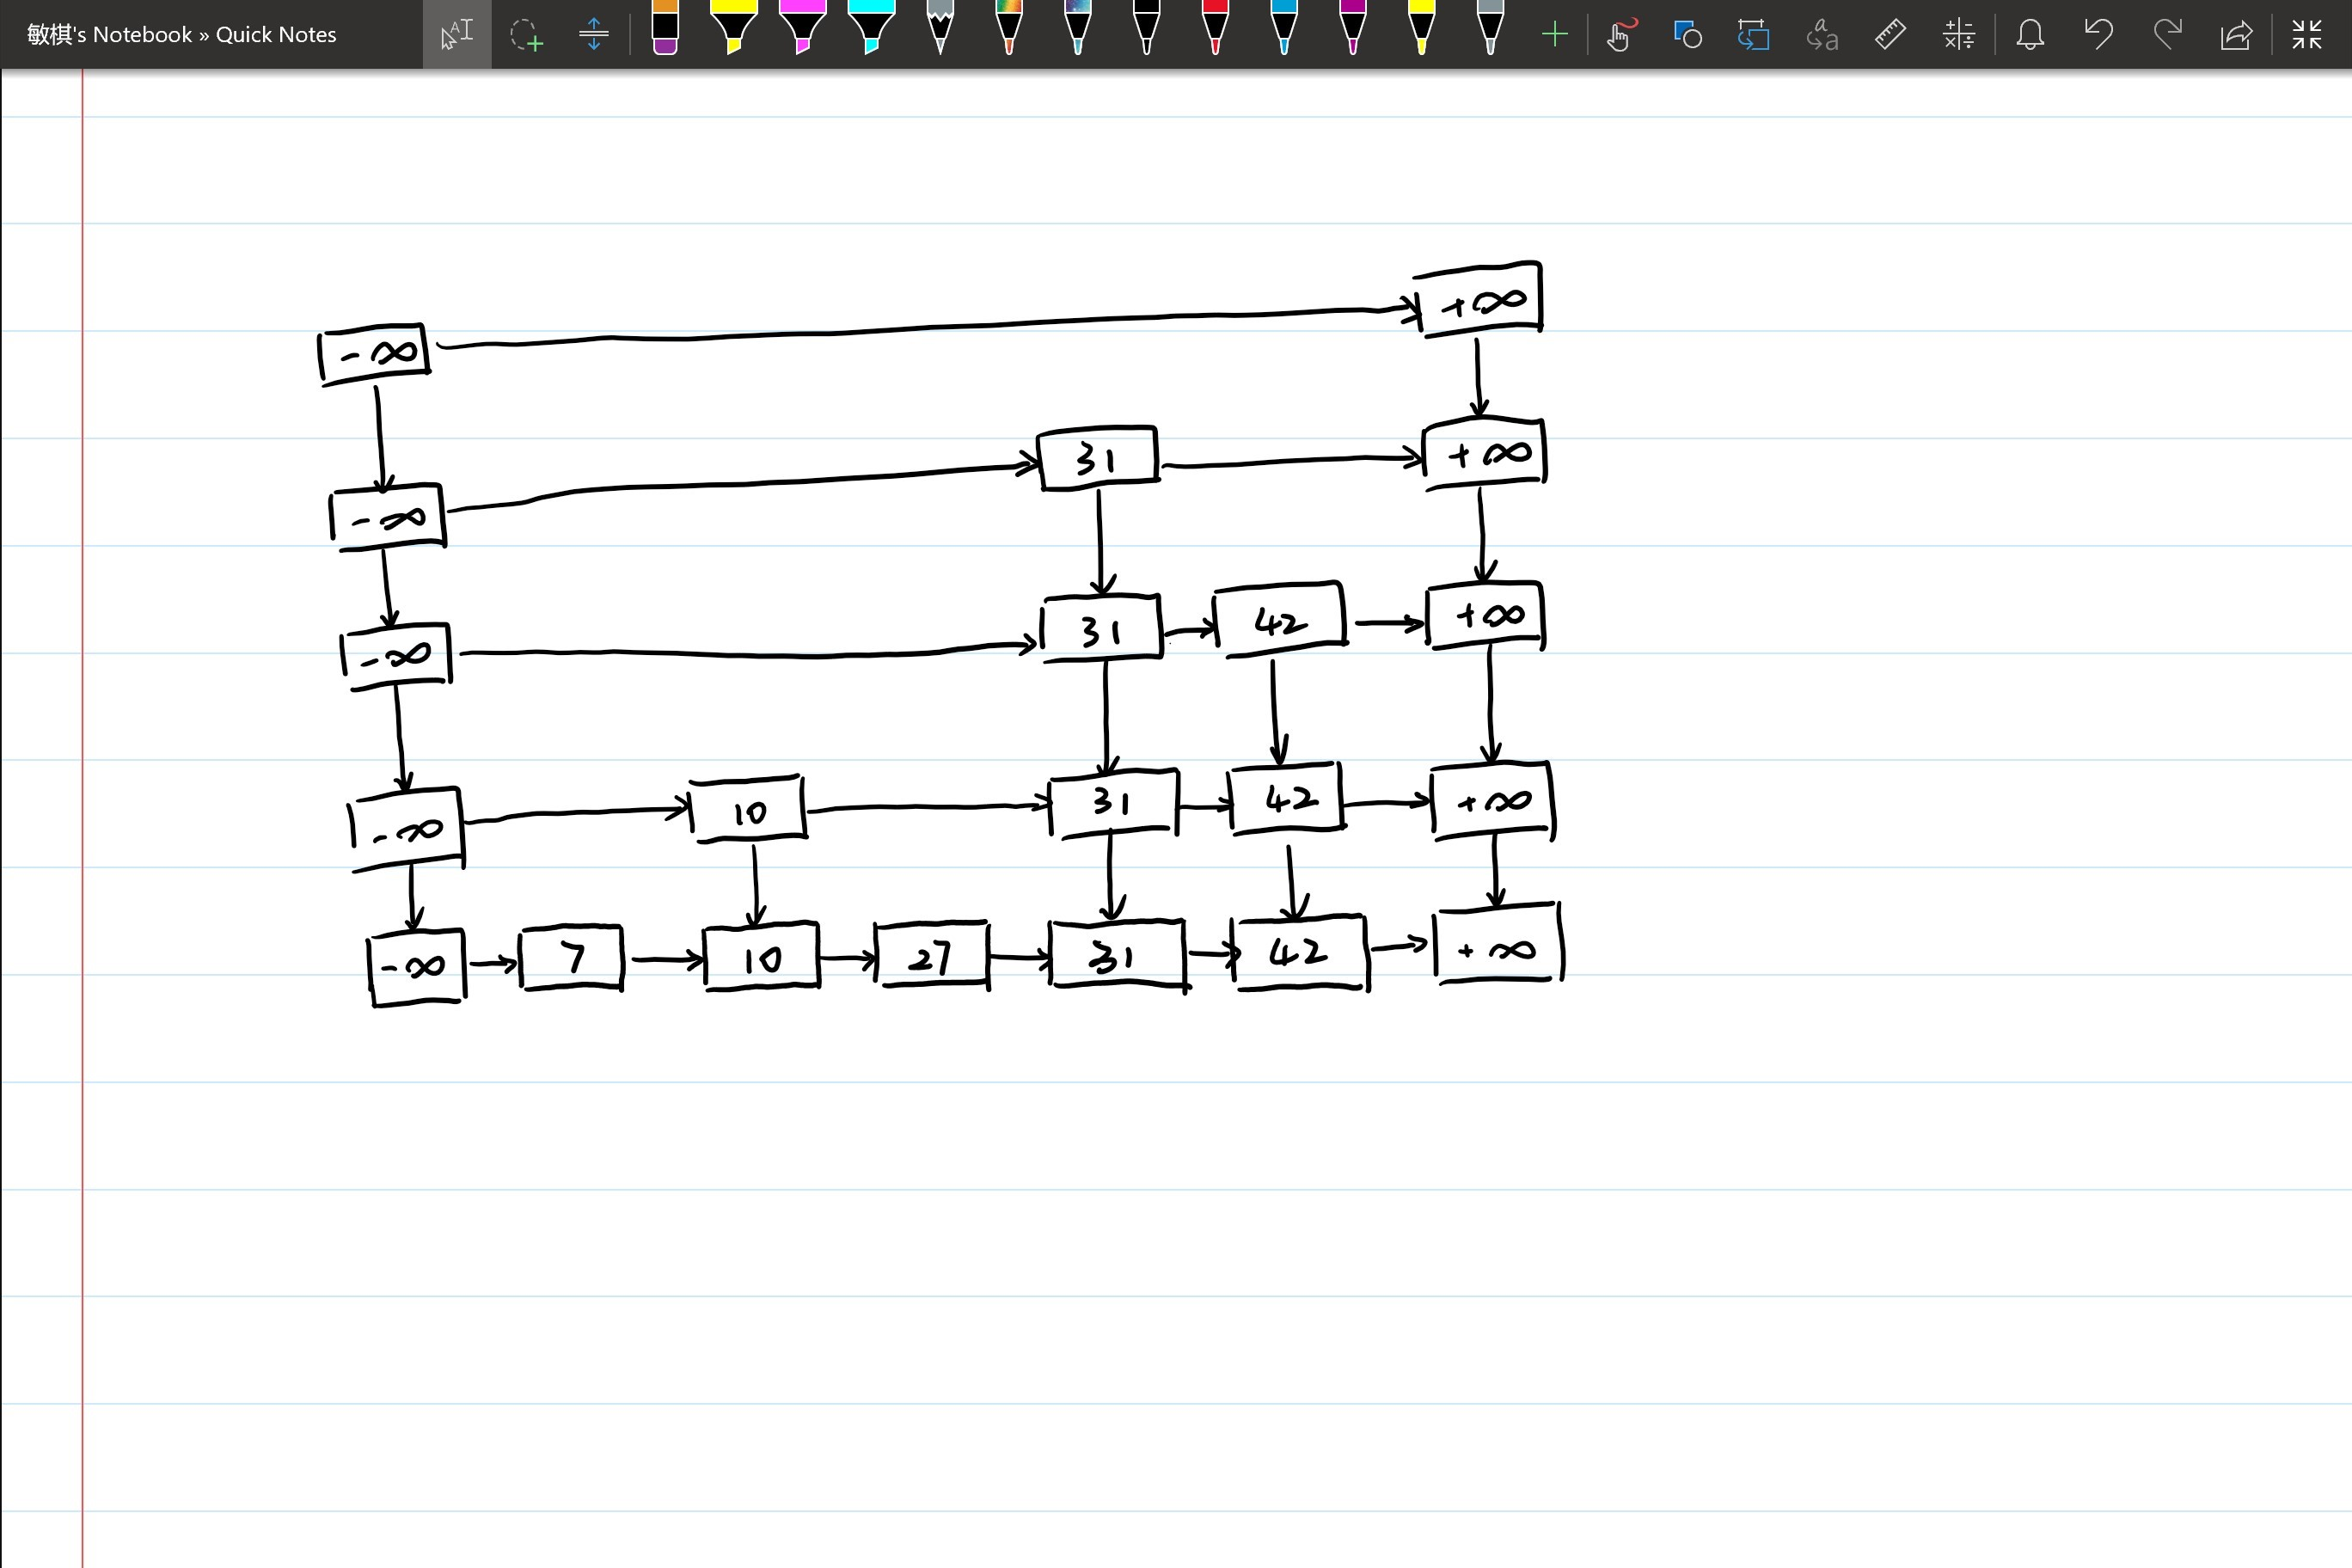
\includegraphics[width=1\textwidth]{7.jpg}
		\end{center}
	\end{figure}
	
	
	b)
	
	A tower of exactly height 3 means that we roll the die, get three 6's consecutively, and at the 4-th time, we get something else.
	
	So the probability should be $\underbrace{\frac{1}{6}^3}_{\text{3 times of 6}} * \underbrace{\frac{5}{6}}_{\text{4th time of else}} = \frac{5}{1296} \approx 0.00386$\\
	
	
	c)
	
	For each key, the probability of increasing the height of tower by 1 is $\frac{1}{6}$
	
	Therefore, for the 1316-key-skiplist, the expected height of tower should be $\log_6 1316$
	
	%%%%%%%%%%%%%%%%%%%%%%%%%%%%%%%%%%%%%%%%%%%%%%%%%%%%%%%%%%%%%
\end{document}